\documentclass{ximera}

\title{Neurale Netwerken}
\author{Mila Vervoort}
\license{CC: 0}         % replace with an appropriate license, or set it in xmPreamble

\begin{document}
\begin{abstract}
    Een introductie over Machine Learning en Neurale Netwerken voor het toepassen op reactorkunde
\end{abstract}
\maketitle
\label{xim: Neurale Netwerken}

\subsection*{Wat is een neuraal netwerk?}

Een \textbf{neuraal netwerk} is een type Machine Learning-model waarmee complexe verbanden tussen invoer- en uitvoergegevens kunnen worden geleerd. Het model is opgebouwd uit verschillende lagen van eenvoudige rekenelementen, die \textbf{neuronen} worden genoemd.

Een neuraal netwerk kan bijvoorbeeld worden gebruikt om een verband van de vorm

\[
\hat{Y}=f_\theta(X)
\]

te leren. Hierbij vormen $X$ de invoergegevens, $\hat{Y}$ de voorspelling van het model en $\theta$ de parameters van het netwerk. Deze parameters worden tijdens het trainen aangepast op basis van de beschikbare gegevens.

In tegenstelling tot een klassieke kinetische vergelijking wordt de exacte vorm van het verband $f_\theta$ niet vooraf opgelegd. Het netwerk krijgt bijvoorbeeld niet de instructie dat een reactiesnelheid van de vorm

\[
r=kC_A^n
\]

moet zijn. In plaats daarvan wordt een voldoende flexibel netwerk gebruikt dat zelf een geschikte relatie tussen de invoer en de uitvoer kan leren.

Een neuraal netwerk wordt daarom vaak beschouwd als een \textbf{black-boxmodel}. We kennen de invoer van het netwerk en kunnen de uiteindelijke uitvoer bekijken, maar de relatie die het netwerk tijdens het trainen leert, is doorgaans veel moeilijker fysisch te interpreteren dan een klassieke vergelijking. De term black box betekent hierbij niet dat er geen model aanwezig is, maar dat de interne werking van het geleerde model moeilijk rechtstreeks te interpreteren is.


\subsection*{Opbouw van een neuraal netwerk}

Een eenvoudig neuraal netwerk bestaat uit een \textbf{inputlaag}, één of meerdere \textbf{hidden layers} en een \textbf{outputlaag}.

\[
\boxed{
\text{Inputlaag}
\rightarrow
\text{Hidden layer(s)}
\rightarrow
\text{Outputlaag}
}
\]

De inputlaag ontvangt de gegevens die aan het model worden aangeboden. De hidden layers verwerken deze gegevens en de outputlaag geeft de uiteindelijke voorspelling van het netwerk. Een netwerk met meerdere hidden layers wordt een \textbf{deep neural network} genoemd. 

\begin{figure}[ht]
\centering

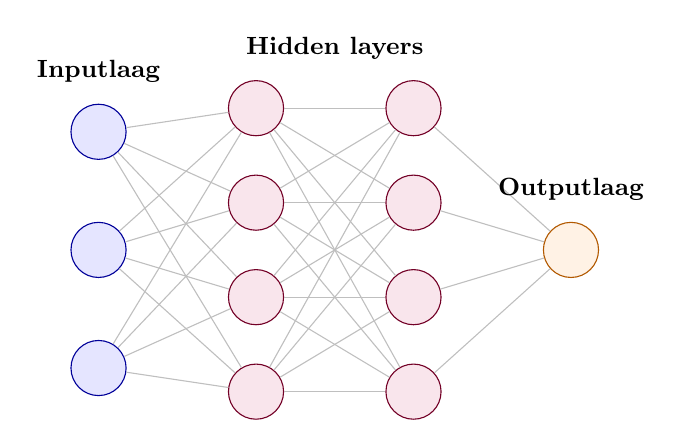
\begin{tikzpicture}[
    neuron/.style={
        circle,
        draw=gray!65!black,
        fill=gray!8,
        minimum size=7mm,
        inner sep=0pt
    },
    input/.style={
        neuron,
        draw=blue!60!black,
        fill=blue!10
    },
    hidden/.style={
        neuron,
        draw=purple!60!black,
        fill=purple!10
    },
    output/.style={
        neuron,
        draw=orange!70!black,
        fill=orange!10
    },
    connection/.style={
        draw=gray!50,
        thin
    }
]

% Inputlaag
\node[input] (x1) at (0,1.5) {};
\node[input] (x2) at (0,0) {};
\node[input] (x3) at (0,-1.5) {};

% Hidden layer 1
\node[hidden] (h11) at (2,1.8) {};
\node[hidden] (h12) at (2,0.6) {};
\node[hidden] (h13) at (2,-0.6) {};
\node[hidden] (h14) at (2,-1.8) {};

% Hidden layer 2
\node[hidden] (h21) at (4,1.8) {};
\node[hidden] (h22) at (4,0.6) {};
\node[hidden] (h23) at (4,-0.6) {};
\node[hidden] (h24) at (4,-1.8) {};

% Outputlaag
\node[output] (y) at (6,0) {};

% Verbindingen
\foreach \i in {x1,x2,x3}
    \foreach \j in {h11,h12,h13,h14}
        \draw[connection] (\i) -- (\j);

\foreach \i in {h11,h12,h13,h14}
    \foreach \j in {h21,h22,h23,h24}
        \draw[connection] (\i) -- (\j);

\foreach \i in {h21,h22,h23,h24}
    \draw[connection] (\i) -- (y);

% Labels
\node[above=5mm, font=\small\bfseries] at (0,1.5)
    {Inputlaag};

\node[above=5mm, font=\small\bfseries] at (3,1.8)
    {Hidden layers};

\node[above=5mm, font=\small\bfseries] at (6,0)
    {Outputlaag};


\end{tikzpicture}

\caption{Schematische voorstelling van een neuraal netwerk.}
\label{fig:neural_network}
\end{figure}


De structuur van een neuraal netwerk bepaalt dus hoe de informatie door het model stroomt. De exacte relatie die het netwerk leert, wordt echter bepaald door de parameters van de neuronen.

\subsection*{Neuronen}

Een neuraal netwerk is opgebouwd uit neuronen. Een neuron ontvangt één of
meerdere invoerwaarden en combineert deze tot één uitvoerwaarde.

Stel dat een neuron de invoerwaarden $x_1,x_2,\ldots,x_n$ ontvangt. Elke
invoer wordt vermenigvuldigd met een \textbf{weight} en vervolgens wordt een
\textbf{bias} opgeteld. Eerst wordt de waarde

\[
z=w_1x_1+w_2x_2+\ldots+w_nx_n+b
\]

berekend. Dit kan compacter worden geschreven als

\[
z=\mathbf{w}^{T}\mathbf{x}+b.
\]

Hierbij zijn $\mathbf{x}$ de invoerwaarden, $\mathbf{w}$ de bijbehorende
weights en $b$ de bias.

De waarde $z$ wordt vervolgens door een \textbf{activatiefunctie} gestuurd.
De uiteindelijke uitvoer van het neuron wordt daarom gegeven door

\[
a=\sigma(z),
\]

waarbij $\sigma$ de activatiefunctie voorstelt.

Een neuron voert dus in essentie twee stappen uit:
\begin{figure}[ht]
\centering
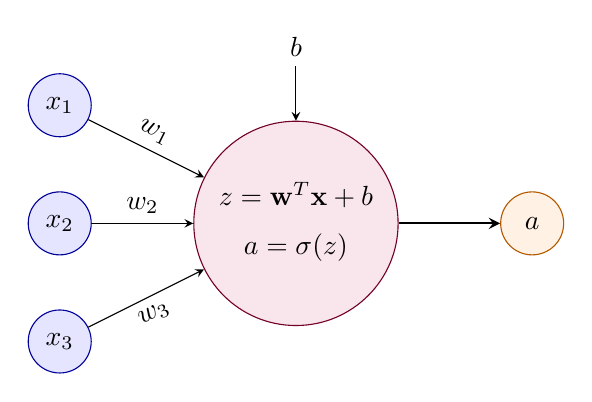
\begin{tikzpicture}[
    >=stealth,
    input/.style={
        circle,
        draw=blue!60!black,
        fill=blue!10,
        minimum size=8mm,
        inner sep=0pt
    },
    neuron/.style={
        circle,
        draw=purple!60!black,
        fill=purple!10,
        minimum size=22mm,
        inner sep=0pt
    },
    output/.style={
        circle,
        draw=orange!70!black,
        fill=orange!10,
        minimum size=8mm,
        inner sep=0pt
    }
]

% Inputs
\node[input] (x1) at (0,1.5) {$x_1$};
\node[input] (x2) at (0,0) {$x_2$};
\node[input] (x3) at (0,-1.5) {$x_3$};

% Neuron
\node[neuron] (n) at (3,0) {
    \begin{tabular}{c}
    $z=\mathbf{w}^T\mathbf{x}+b$\\[2mm]
    $a=\sigma(z)$
    \end{tabular}
};

% Output
\node[output] (a) at (6,0) {$a$};

% Connections
\draw[->] (x1) -- node[above,sloped] {$w_1$} (n);
\draw[->] (x2) -- node[above] {$w_2$} (n);
\draw[->] (x3) -- node[below,sloped] {$w_3$} (n);

\draw[->, thick] (n) -- (a);

% Bias
\draw[->] (3,2.0) 
    node[above] {$b$}
    -- (n.north);

\end{tikzpicture}

\caption{Schematische voorstelling van één neuron. De invoerwaarden worden
gewogen en opgeteld met een bias, waarna een activatiefunctie wordt toegepast.}
\label{fig:single_neuron}
\end{figure}


De activatiefunctie bepaalt hoe de waarde $z$ wordt omgezet naar de uitvoer
$a$. Enkele veelgebruikte activatiefuncties zijn de sigmoidfunctie, de
hyperbolische tangens en de ReLU-functie:

\[
\begin{aligned}
\text{sigmoid:}\qquad
&\sigma(z)=\frac{1}{1+e^{-z}},
&&0<\sigma(z)<1,\\[2mm]
\text{tanh:}\qquad
&\tanh(z)=\frac{e^z-e^{-z}}{e^z+e^{-z}},
&&-1<\tanh(z)<1,\\[2mm]
\text{ReLU:}\qquad
&\operatorname{ReLU}(z)=\max(0,z),
&&\operatorname{ReLU}(z)\geq0.
\end{aligned}
\]

De sigmoidfunctie zet de waarde $z$ dus om naar een waarde tussen $0$ en
$1$, terwijl tanh waarden tussen $-1$ en $1$ geeft. De ReLU zet negatieve
waarden op nul en laat positieve waarden ongewijzigd.

Deze activatiefuncties zorgen voor \textbf{niet-lineariteit} in het netwerk.
Zonder activatiefuncties zouden meerdere opeenvolgende lineaire lagen
uiteindelijk samen slechts één lineaire transformatie vormen. Door
niet-lineaire activatiefuncties te gebruiken, kan een neuraal netwerk
complexere, niet-lineaire verbanden leren.

De \textbf{weights} en \textbf{biases} zijn de trainbare parameters van het
neuron. De weights bepalen hoe sterk de verschillende invoerwaarden
bijdragen aan $z$, terwijl de bias de waarde van $z$ verschuift. Tijdens het
trainen worden deze parameters aangepast om de voorspellingen van het
netwerk te verbeteren.




\begin{question}
\text{Hoeveel trainbare parameters heeft dit netwerk?}

Beschouw het onderstaande neurale netwerk:

\begin{center}
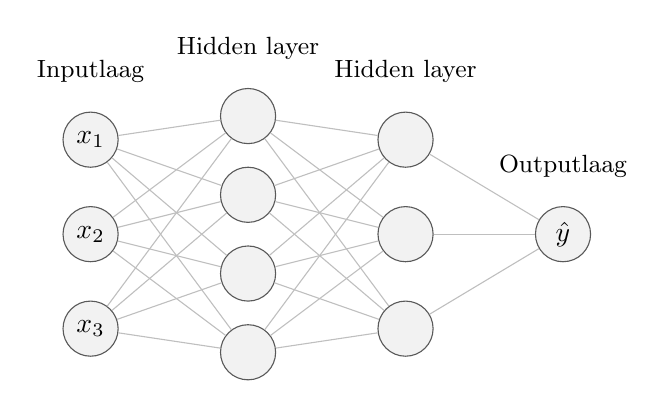
\begin{tikzpicture}[
    neuron/.style={
        circle,
        draw=gray!70!black,
        fill=gray!10,
        minimum size=7mm,
        inner sep=0pt
    },
    >=stealth
]

% Inputlaag
\node[neuron] (x1) at (0,1.2) {$x_1$};
\node[neuron] (x2) at (0,0) {$x_2$};
\node[neuron] (x3) at (0,-1.2) {$x_3$};

% Hidden layer 1
\node[neuron] (h11) at (2,1.5) {};
\node[neuron] (h12) at (2,0.5) {};
\node[neuron] (h13) at (2,-0.5) {};
\node[neuron] (h14) at (2,-1.5) {};

% Hidden layer 2
\node[neuron] (h21) at (4,1.2) {};
\node[neuron] (h22) at (4,0) {};
\node[neuron] (h23) at (4,-1.2) {};

% Outputlaag
\node[neuron] (y) at (6,0) {$\hat{y}$};

% Verbindingen
\foreach \i in {x1,x2,x3}
    \foreach \j in {h11,h12,h13,h14}
        \draw[gray!50] (\i) -- (\j);

\foreach \i in {h11,h12,h13,h14}
    \foreach \j in {h21,h22,h23}
        \draw[gray!50] (\i) -- (\j);

\foreach \i in {h21,h22,h23}
    \draw[gray!50] (\i) -- (y);

% Labels
\node[above=3mm] at (0,1.5) {\small Inputlaag};
\node[above=3mm] at (2,1.8) {\small Hidden layer};
\node[above=3mm] at (4,1.5) {\small Hidden layer};
\node[above=3mm] at (6,0.3) {\small Outputlaag};

\end{tikzpicture}
\end{center}

Elk neuron in de hidden layers en de outputlaag heeft één bias. Elke
verbinding tussen twee neuronen heeft één weight.

Hoeveel \textbf{trainbare parameters} heeft dit netwerk in totaal?

\[
N_{\mathrm{parameters}}
=
\answer{41}
\]

\begin{feedback} \text{ }

De parameters bestaan uit de \textbf{weights} en de \textbf{biases}.

Om het aantal weights te bepalen, kijken we naar de verbindingen tussen
opeenvolgende lagen. Elk neuron in een volgende laag ontvangt een weight
van elk neuron in de vorige laag.

Tussen de inputlaag met $3$ neuronen en de eerste hidden layer met $4$
neuronen zijn er daarom $3\times4=12$ weights. Elk van de $4$ neuronen in de eerste hidden layer is immers
verbonden met alle $3$ inputneuronen.
Tussen de eerste hidden layer en de tweede hidden layer zijn er $4\times3=12$ weights en tussen de tweede hidden layer zijn er $3\times1=3$ weights.

Er zijn in totaal dus \[3\times4+4\times3+3\times1=33\]
weights.

Daarnaast heeft elk neuron in de hidden layers en de outputlaag één bias.
Er zijn dus
\[
N_{\mathrm{biases}}
=
4+3+1
=
8
\]

biases.

Het totale aantal trainbare parameters is dus
\[
N_{\mathrm{parameters}}
=
33+8
=
\boxed{41}.
\]
    
\end{feedback}
\end{question}

\subsection*{Forward propagation}

Wanneer gegevens aan een neuraal netwerk worden aangeboden, worden deze
stap voor stap door de verschillende lagen verwerkt. Dit proces noemen we
\textbf{forward propagation}.

Voor een netwerk met $L$ lagen wordt de uitvoer van iedere laag berekend op
basis van de uitvoer van de vorige laag. Voor laag $l$ geldt:

\[
z^{[l]}
=
W^{[l]}a^{[l-1]}+b^{[l]},
\]
\[
a^{[l]}
=
g^{[l]}\left(z^{[l]}\right).
\]

waarbij $W^{[l]}$ de weights van laag $l$ bevat, $b^{[l]}$ de biases zijn en
$a^{[l-1]}$ de uitvoer van de vorige laag is.

Voor een netwerk met bijvoorbeeld twee hidden layers en een outputlaag
verloopt de berekening dus als volgt:
\[
\boxed{
\begin{aligned}
z^{[1]} &= W^{[1]}x+b^{[1]}, &
a^{[1]} &= g^{[1]}(z^{[1]}),\\[2mm]
z^{[2]} &= W^{[2]}a^{[1]}+b^{[2]}, &
a^{[2]} &= g^{[2]}(z^{[2]}),\\[2mm]
z^{[3]} &= W^{[3]}a^{[2]}+b^{[3]}, &
\hat{y} &= a^{[3]}.
\end{aligned}
}
\]

Op deze manier wordt de informatie achtereenvolgens door het netwerk verwerkt totdat de uiteindelijke voorspelling $\hat{y}$ wordt verkregen.

Schematisch kan dit worden voorgesteld als

\begin{figure}[ht]
\centering

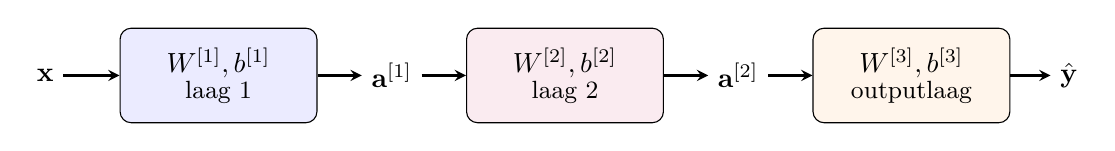
\begin{tikzpicture}[
    >=stealth,
    box/.style={
        draw,
        rounded corners,
        minimum height=12mm,
        minimum width=25mm,
        align=center
    }
]

\node (x) at (0,0) {$\mathbf{x}$};

\node[box, fill=blue!8] (l1) at (2.2,0)
    {$W^{[1]},b^{[1]}$\\[-1mm]\small laag 1};

\node (a1) at (4.4,0) {$\mathbf{a}^{[1]}$};

\node[box, fill=purple!8] (l2) at (6.6,0)
    {$W^{[2]},b^{[2]}$\\[-1mm]\small laag 2};

\node (a2) at (8.8,0) {$\mathbf{a}^{[2]}$};

\node[box, fill=orange!8] (l3) at (11,0)
    {$W^{[3]},b^{[3]}$\\[-1mm]\small outputlaag};

\node (y) at (13,0) {$\hat{\mathbf y}$};

\draw[->, thick] (x) -- (l1);
\draw[->, thick] (l1) -- (a1);
\draw[->, thick] (a1) -- (l2);
\draw[->, thick] (l2) -- (a2);
\draw[->, thick] (a2) -- (l3);
\draw[->, thick] (l3) -- (y);

\end{tikzpicture}

\caption{Schematische voorstelling van forward propagation door een neuraal
netwerk.}
\label{fig:forward_propagation}
\end{figure}


\subsection*{Het trainen van een neuraal netwerk}

Om een neuraal netwerk bruikbaar te maken, moeten de weights en biases van het
netwerk worden geleerd uit beschikbare gegevens. Tijdens het trainen worden
deze parameters zo aangepast dat de voorspellingen van het netwerk steeds
beter overeenkomen met de gewenste uitvoer.

\subsubsection*{De lossfunctie}

Om te bepalen hoe goed het netwerk voorspelt, vergelijken we de voorspelling
$\hat{Y}$ met de gewenste waarde $Y$. Hiervoor gebruiken we een
\textbf{lossfunctie} of \textbf{kostfunctie}. De loss geeft aan hoe groot de
fout van het netwerk is.

Een veelgebruikte lossfunctie voor regressie is de
\textbf{Mean Squared Error} (MSE):

\[
\mathrm{MSE}
=
\frac{1}{N}
\sum_{i=1}^{N}
\left(
Y_i-\hat{Y}_i
\right)^2.
\]

Een kleine waarde van de loss betekent dat de voorspellingen gemiddeld dicht bij de gewenste waarden liggen. Het doel van het trainen is daarom om de parameters van het netwerk zo aan te passen dat de loss zo klein mogelijk wordt.

\subsubsection*{Backpropagation}

Tijdens het trainen wordt eerst via \textbf{forward propagation} een
voorspelling $\hat{Y}$ gemaakt. Vervolgens wordt de loss berekend. Om de
parameters van het netwerk aan te kunnen passen, moeten we bepalen hoe sterk
iedere parameter bijdraagt aan de loss.

Dit gebeurt met \textbf{backpropagation}. Backpropagation berekent de
gradiënten van de loss naar de verschillende weights en biases. Voor de
parameters van laag $l$ zijn dit bijvoorbeeld

\[
\frac{\partial L}{\partial W^{[l]}}
\qquad\text{en}\qquad
\frac{\partial L}{\partial b^{[l]}}.
\]

Deze gradiënten geven aan hoe sterk de loss verandert wanneer de
desbetreffende parameters worden aangepast.

Een belangrijk onderdeel van backpropagation is de \textbf{kettingregel}.
Omdat de uitvoer van een laag de invoer van de volgende laag vormt, kan de
invloed van een parameter op de uiteindelijke loss worden bepaald door de
invloeden door de opeenvolgende lagen heen te combineren.

Voor één parameter $\theta$ kan dit schematisch worden voorgesteld als

\[
\theta
\rightarrow
z
\rightarrow
a
\rightarrow
\hat{y}
\rightarrow
L.
\]

Met de kettingregel wordt dan

\[
\boxed{
\frac{\partial L}{\partial \theta}
=
\frac{\partial L}{\partial \hat{y}}
\frac{\partial \hat{y}}{\partial a}
\frac{\partial a}{\partial z}
\frac{\partial z}{\partial \theta}
}
\]

Backpropagation voert deze berekening efficiënt uit voor de verschillende
parameters van het netwerk.

\subsubsection*{Aanpassen van de parameters}

De berekende gradiënten worden vervolgens gebruikt om de weights en biases aan te passen. Een eenvoudige methode hiervoor is \textbf{gradient descent}. Hierbij worden de parameters aangepast volgens

\[
\boxed{
\theta
\leftarrow
\theta-\eta\nabla_\theta L
}
\]

waarbij $\theta$ de netwerkparameters zijn, $L$ de lossfunctie en $\eta$ de \textbf{learning rate}. De learning rate bepaalt hoe groot de stap is waarmee de parameters worden aangepast.

Het minteken zorgt ervoor dat de parameters worden aangepast in de richting waarin de loss afneemt.

In de praktijk wordt vaak een variant van gradient descent gebruikt, zoals de \textbf{Adam}-optimizer. Adam gebruikt naast de huidige gradiënten ook informatie uit eerdere gradiënten om de parameterupdates aan te passen.


\subsubsection*{Het volledige trainingsproces}

Het trainen van een neuraal netwerk bestaat dus uit een herhaald proces:

\[
\boxed{
\begin{array}{c}
\text{Forward propagation}\\
\downarrow\\
\text{Voorspelling } \hat{Y}\\
\downarrow\\
\text{Loss berekenen}\\
\downarrow\\
\text{Backpropagation}\\
\downarrow\\
\text{Gradiënten berekenen}\\
\downarrow\\
\text{Parameters aanpassen}\\
\downarrow
\\[-1mm]
\text{opnieuw}
\end{array}
}
\]

Bij iedere trainingsstap worden de weights en biases dus aangepast op basis van de berekende loss en gradiënten. Door dit proces herhaald uit te voeren, kan het netwerk een steeds betere relatie tussen de invoer en de gewenste uitvoer leren.

\subsubsection*{Neurale netwerken in de reactorkunde}

In de vorige secties werd besproken hoe machine learning en neurale netwerken kunnen worden gebruikt om verbanden uit experimentele gegevens te leren. We kunnen dit principe nu toepassen op een reactiesysteem in een batchreactor.

Stel dat we een batchreactor onderzoeken waarin verschillende componenten met elkaar reageren. Tijdens een experiment meten we op verschillende tijdstippen de concentraties van de aanwezige componenten. We verkrijgen bijvoorbeeld concentratieprofielen van de vorm: $C_A(t), C_B(t), C_C(t)$. 

Bij de eerder besproken methodes (integrale analysemethode, ...) probeerden we telkens een geschikte kinetische vergelijking te vinden en vervolgens bepaalden we de onbekende kinetische parameters. Bij een data-driven benadering hoeven we echter niet vooraf een specifieke vorm voor de reactiesnelheid te kiezen. In plaats daarvan laten we een neuraal netwerk leren hoe de toestand van het reactiesysteem verandert.

De toestand van het reactiesysteem kan worden beschreven met de concentratievector
\[
\mathbf{C} =
\begin{pmatrix}
C_A \\
C_B \\
C_C
\end{pmatrix}.
\]

Het neurale netwerk krijgt deze concentraties als invoer. De uitvoer van het netwerk bestaat uit de overeenkomstige veranderingen van de concentraties:
\[
\frac{d\mathbf{C}}{dt}
=
\text{neuraal netwerk}(\mathbf{C}).
\]


Het netwerk leert dus een functie
\[
\frac{d\mathbf{C}}{dt} = f_\theta(\mathbf{C}),
\]
waarbij \(f_\theta\) de functie is die door het neurale netwerk wordt voorgesteld en \(\theta\) de trainbare parameters van het netwerk bevat.

Voor drie componenten betekent dit concreet:
\[
f_\theta
\begin{pmatrix}
C_A \\
C_B \\
C_C
\end{pmatrix}
=
\begin{pmatrix}
\dfrac{dC_A}{dt} \\
\dfrac{dC_B}{dt} \\
\dfrac{dC_C}{dt}
\end{pmatrix}.
\]

Het netwerk probeert dus te leren hoe snel de verschillende concentraties veranderen wanneer het systeem zich in een bepaalde toestand bevindt. Deze informatie over de lokale concentratieveranderingen kunnen we vervolgens gebruiken om te bepalen hoe het volledige reactiesysteem zich in de tijd ontwikkelt. 

Uiteindelijk willen we opnieuw een concentratieprofiel verkrijgen, $\mathbf{C}(t)$, omdat dit de grootheid is die we experimenteel hebben gemeten en waarmee we de voorspelling van het model kunnen vergelijken. Om dit profiel te verkrijgen, moeten de door het neurale netwerk voorspelde afgeleiden $\frac{d\mathbf{C}}{dt}$ over de tijd worden geïntegreerd.

Om dit te doen, moeten we de differentiaalvergelijking

\[
\frac{d\mathbf{C}}{dt} = f_\theta(\mathbf{C})
\]
oplossen met een gekende beginconditie
$\mathbf{C}(t_0) = \mathbf{C}_0$.

Hiervoor gebruiken we een ODE-oplosser. Deze gebruikt de door het neurale netwerk voorspelde concentratieveranderingen om stap voor stap te berekenen hoe de concentraties in de tijd evolueren.

We verkrijgen zo een voorspeld concentratieprofiel $\mathbf{C}_{\mathrm{pred}}(t)$, dat we kunnen vergelijken met het experimenteel gemeten concentratieprofiel
$\mathbf{C}_{\mathrm{exp}}(t).$

Uit het verschil tussen deze twee profielen wordt de loss berekend.  Vaak wordt hiervoor de Mean Squared Error (MSE) gebruikt: 

\[
\mathcal{L}
=
\frac{1}{N}
\sum_{i=1}^{N}
\left\|
\mathbf{C}_{\mathrm{pred}}(t_i)
-
\mathbf{C}_{\mathrm{exp}}(t_i)
\right\|^2.
\]

Vervolgens worden via backpropagation de gradiënten van deze loss ten opzichte van de netwerkparameters berekend. De optimizer past de parameters van het netwerk vervolgens aan.

Het volledige leerproces kan daarom als volgt worden weergegeven:

\[
\begin{array}{c}
\text{Experimentele concentratieprofielen}
\\
\downarrow
\\
\text{Neuraal netwerk}
\\
\downarrow
\\
\text{Voorspelde } \dfrac{d\mathbf{C}}{dt}
\\
\downarrow
\\
\text{ODE-oplosser}
\\
\downarrow
\\
\text{Voorspelde concentratieprofielen}
\\
\downarrow
\\
\text{Vergelijking met experiment}
\\
\downarrow
\\
\text{Loss}
\\
\downarrow
\\
\text{Backpropagation + Optimizer}
\\
\downarrow
\\
\text{Nieuwe netwerkparameters}
\end{array}
\]

Dit proces wordt vervolgens vele malen herhaald. Na elke iteratie worden de netwerkparameters aangepast, zodat het voorspelde concentratieprofiel steeds beter overeenkomt met de experimentele gegevens.


Na het trainen hebben we dus geen klassieke kinetische vergelijking zoals $r = k C_A^n$ met een beperkt aantal interpreteerbare parameters \(k\) en \(n\). In plaats daarvan hebben we een neuraal netwerk dat voor een gegeven toestand van het reactiesysteem een voorspelling maakt van de lokale verandering van de concentraties.

Bijvoorbeeld:

\[
\begin{pmatrix}
C_A \\
C_B \\
C_C
\end{pmatrix}
=
\begin{pmatrix}
0.8 \\
0.1 \\
0.1
\end{pmatrix}
\quad
\xrightarrow{\text{NN}}
\quad
\begin{pmatrix}
\dfrac{dC_A}{dt} \\
\dfrac{dC_B}{dt} \\
\dfrac{dC_C}{dt}
\end{pmatrix}.
\]

Het netwerk kan dus worden gebruikt om te voorspellen hoe het systeem vanuit die toestand verder evolueert.

Dit betekent echter niet dat het netwerk automatisch een universeel kinetisch model van de reactie heeft gevonden. Het heeft geleerd van de toestanden die in de beschikbare experimentele gegevens voorkomen. Voorspellingen buiten het gebied waarin het netwerk werd getraind, kunnen daarom onbetrouwbaar zijn.



\end{document}